\documentclass[fleqn,10pt]{wlscirep}
\usepackage[T1]{fontenc}
\usepackage{lineno}
\linenumbers
% \documentclass[a4paper,10pt]{article}
\usepackage[utf8]{inputenc}
\usepackage{authblk}
\usepackage{tabularx}
\usepackage{url}
\usepackage{graphicx}
\graphicspath{{images/}}
\usepackage{caption}
\usepackage{subcaption}
\usepackage{multirow}
\usepackage{multicol}
\usepackage{listings}
\usepackage{placeins}

\title{SuperMat: Construction of a linked annotated dataset from superconductors-related literature}

\author[1*]{Luca Foppiano}
\author[1]{Sae Dieb}
\author[1]{Akira Suzuki}
\author[2]{Pedro Baptista de Castro}
\author[2]{Suguru Iwasaki}
\author[2]{Azusa Uzuki}
\author[2]{Miren Garbine Esparza Echevarria}
\author[2]{Yan Meng}
\author[2]{Kensei Terashima}
\author[3]{Laurent Romary}
\author[2]{Yoshihiko Takano}
\author[1*]{Masashi Ishii}

\affil[1]{Material Database Group, MaDIS, NIMS, Tsukuba, 305-0011, Japan}
\affil[2]{Nano Frontier Superconducting Materials Group, MANA, NIMS, Tsukuba, 305-0011, Japan}
\affil[3]{ALMAnaCH, Inria, Paris, 75012, France}

\affil[*]{corresponding author(s): Luca Foppiano (FOPPIANO.Luca@nims.go.jp), Masashi Ishii (ISHII.Masashi@nims.go.jp)}


\begin{abstract}

% importance of text and data mining in material research (max 2 sentences) 
In materials science, abundant publications are available as knowledge sources, although not usable as machine-readable media.
The development of text and data mining (TDM) processes is necessary to exploit this prosperity of information. 
Scientists can benefit from this information overloading, for example, in material discovery data driven computation may suggest novel materials with desired physical properties. 
Superconductors materials are already used in many applications, and the research is still active.
%% What we did 
In this paper, we present SuperMat (Superconductor Materials) a new annotated dataset of linked data from superconductors scientific literature. 
SuperMat, composed of 145 articles and 9966 entities (or which, 4000 unique) [TODO: update figures], contains annotations of materials and samples, classes, properties (superconducting critical temperature, measurement method), and conditions (applied pressure). 
Additionally, the dataset provides links between entities: materials and their respective superconducting critical temperature (\textit{T\textsubscript{c}}), their parametric conditions such as applied pressure or methods of measurements, when specified.
% How we did it 
This work is the result of a fruitful collaboration between computers- and material- scientists and includes the dataset, the annotation guidelines and the annotation support tools.
Our methodology follows four steps: (1) relevant information selection, (2) tag-set design, (3) annotation rules definitions, and (4) annotation process.
% What we found out 
We ensure proper quality through validation by domain experts. We reduced the human annotation errors with the adoption of annotations supports tools. 
We verified the reliability of the annotation guidelines by reaching a satisfying Inter Annotator Agreement (IAA) by novice annotators with general materials science knowledge autonomously.
% What we conclude
SuperMat can be used to support TDM processes for many complementary tasks such as information retrieval, entity extraction, entity linking, and information clustering.

% The dataset can bee utilised this dataset to train a sequence labelling system, which was then applied to semantically enhance a search engine for scientific documents and a document classification system using superconductors-related classes. 
\end{abstract}

\begin{document}
\flushbottom
\maketitle



\section*{Background and summary}
% Introduction, why text is important for scientific knowledge? 
The vast majority of scientific knowledge is available, with overwhelming abundance~\cite{Grigas2017JustGI, Khabsa2014TheNO, OrduaMalea2015MethodsFE, Bjrk2009ScientificJP} through published papers and articles. 
However, most of the information is presented as text, which is an arbitrary and unstructured form of communication, challenging to be used as machine-readable media. 
% TDM and its importance - next sentence needs to link the a) abundance, and b) unstructured with the end result (structured data) -> TDM For the win... 

The computer-assisted process for identifying and collecting information from scientific literature also referred to as text and data mining (TDM), is a supportive asset for scientific research. 
In the past decades, TDM processes have evolved their ability to perform automatic document processing such as information retrieval, entity extraction, and clustering in several natural sciences.  
%The establishment of Text and Data Mining (TDM) processes is an unavoidable step to bridge information collected from scientific literature toward data-driven discovery. 

% Practical example in biology 
For example, in biology, TDM has been applied in information extraction to identify agents interaction (e.g. bacteria, virus, genes, proteins)~\cite{10.1371/journal.pone.0004554, Krallinger2010, Krallinger2009ExtractionOH} or to support the research against serious diseases, like cancer~\cite{Krasnitz2019CancerB}. 
Chemical compounds name disambiguation, synthesis extraction and retrieval, are other applications in chemistry~\cite{Hawizy2011ChemicalTaggerAT}.

These applications utilised manually curated datasets (corpora) as infrastructures for their TDM systems. For example, BioCreative IV CHEMDNER corpus~\cite{Krallinger2015TheCC} in chemistry, and Genia~\cite{Kim2003GENIAC} and GENETAG~\cite{Tanabe2005GENETAGAT, Ohta2009IncorporatingGA} in biology. The availability of such datasets is a crucial requirement for developing, training, and evaluating TDM systems.

In materials science domain, however, there are only very limited such resources. We can mention NaDev~\cite{Dieb2016} to support the research of nanocrystal devices and, a material-synthesis corpus, for extracting synthesis recipes~\cite{kononova_text-mined_2019}. Materials scientists rely on theoretical approaches such as Density Functional Theory (DFT) or ab-initio calculations , often based on manually extracted data. 
The adoption of data-driven computation (today called Materials Informatics (MI)) had been facing several challenges: lack of data standard, difficulty to understand the practical data-driven applicability, a wide variety of conflicting stack-holders, and missing incentives to contribute to large collaborative initiatives~\cite{Hill2016MaterialsSW}. It is necessary to fill this gap by creating infrastructural resources in materials science to support TDM process. For example, such datasets can support automatic construction of databases for materials and their properties. Such application can save the cost of manually reading the new papers to pick up the newly reported materials and their properties. Additionally, and equally important, it enables scientists to focus and leverage computing power for finding deeper relationships between information potentially unrelated. Another examples include providing semantically enriched search engines able to accept fine-grain queries~\cite{Liu2019SurfaceMR} to reduce the time needed looking for information. 
All these processes cannot be easily established without essential resources like dictionaries, lexicons, datasets. 

% Superconductors domain
Superconductors show a number of characteristic phenomena such as \textit{zero-resistivity}, which can host high magnetic field, quantization of flux inside the superconducting loop, vortex pinning, and so on.  Therefore, they have many promising applications from daily-life to fundamental research. For instance, they are already present in medical devices, high-speed trains, quantum computers, and in the Linear Hadron Collider (LHC)~\cite{PhilippeBook, Kizu2010ConstructionOT, Cardani2017NewAO}. 
However, to discover a new superconductor is very difficult, it is said that only 3\% of candidate materials is, in practice, a superconductor~\cite{Konno2018DeepLO}.
The available resources to support such discovery are still very limited. For example, the National Institute for Materials Science (NIMS) in Japan has been manually constructing databases to support materials research, and SuperCon\footnote{\url{http://supercon.nims.go.jp}} was a hopeful data source for superconductor domain. 
%%[How Supercon is supposed support material research]
Its data aims to support the development of  superconducting critical temperature prediction systems (\textit{T\textsubscript{c}})~\cite{stanev2017machine}. Potentially, it can leverage processes for designing new materials with higher \textit{T\textsubscript{c}}, ideally up to room temperature~\cite{Hamlin2019SuperconductivityNR}. One way to support superconductors research is to increase and enrich the available data (Supercon, for example).

In this paper, we present SuperMat (Superconductors Materials), our inter-disciplinary work for creating a linked annotated dataset for superconductor material data. This dataset contains linked information that can serves as an infrastructural data to support the development of new TDM processes for the superconductors domain. 

%[Summarise the approach]
The annotated information was selected in collaboration with domain experts. 
A preliminary annotation study on a small number of papers was conducted for domain exploration. We bootstrap the guidelines to annotate this information, and to design an annotation process.
Based on this preliminary study, we designed the tag-sets and validated it with domain-experts. 

We collected papers related to research in superconductivity from different sources and publishers.  
We followed the iterative annotation process of five steps: a) data preparation, b) annotation of relevant entities, c) validation of the annotated data by domain experts, d) test and evaluation, and e) review. The annotation guidelines received updates at every iteration. 
We measured the Inter Annotation Agreement (IAA) using the Krippendorff alpha coefficient~\cite{Krippendorff2004ReliabilityIC} between the intermediate (b) and the final validated data (c). We studied the results obtained from users divided by the level of domain knowledge (domain-experts and non-domain experts) and annotation expertise (novices vs experienced). 
We reached a satisfying average agreement above 0.8 (Section \ref{sec:technical-validation}). 
We measured the reliability  of the guidelines by reporting that novices annotators with general materials science knowledge could reach a satisfying Inter Annotator Agreement (IAA) in autonomy.

As a result, we achieved a dataset composed of 145 articles, with 9966 entities (of which, about 4000 unique entities) [TODO: update figures]. They were annotated using six classes, described in details in Section~\ref{sec:method}: material, class, critical temperature expressions, critical temperature value, critical pressure value and measurement method.
We added a layer of links between entities, of three types: 1) \textit{material-tc} linking materials and their respective superconducting critical temperature \textit{T\textsubscript{c}}. 
2) \textit{tc-pressure} connecting \textit{T\textsubscript{c}} and the applied pressure at which it was obtained, and 3) \textit{tc-me\_method} between the critical temperature with the method used to obtain the value of \textit{T\textsubscript{c}}. 
%The superconducting critical temperature is susceptible to conditions such as magnetic field or pressure. 

% usage of dataset
SuperMat can be used to develop TDM processes for achieving several complementary tasks: 
1) creation of an automatic system for dataset creation, 
2) articles classification, 
3) named entity extraction, for example, automatic dictionaries construction, 
4) clustering and document synthesis,
5) training of Machine Learning (ML) algorithms,
6) evaluation of rules-based or ML-based algorithms, and 
7) development of downstream processes, such as material name parser, or quantities normalisation.


The data structure, comprising classes of materials, materials names and the related properties, is common among different domains in materials science. 
SuperMat can be reused to facilitate or bootstrap the creation of new TDM processes on domains in materials science, other than superconductors research.

%Entity reusability
In the case of entity extraction, for example, a trained Named Entities Recognition (NER) model, trained with SuperMat could recognise materials formulas that are mentioned in the text, on other domains, such as piezoelectric, magnetocaloric, and thermoelectric research.
The process could be further improved by fine-tuning by simply adding new data, or to utilise techniques of transfer learning. 

% Linking reusability
The links between entities, on the other hand, can be utilised in a more general extends to implement and evaluate tasks of Entity Linking (EL) having the goal of extract relationships between properties and materials. 
Contrary to NER, this task is less dependent to domain variability because, intuitively, the structure of the sentences between entities is homogeneous.
As an example, in polymer research, while a NER model trained on SuperMat will not perform well because of the completely different structure of the polymers names, its linked entities can provide training or evaluation data for developing techniques for linking polymers and their respective properties.

In this article, we present SuperMat, a new dataset of linked annotated data of superconductors materials and their properties. SuperMat aims to establish a solid foundation where to build and improve TDM processes in superconducting materials science.
Our contribution consists of the annotated and linked dataset, the guidelines and the methodology we have described in this article, we hope can support other researchers to create annotated data systematically.

In future, we plan to utilise this dataset as training data for an automatic database creation system focusing on superconducting materials and their respective properties. 
The unique feature of links between entities will allow to develop, adapt or evaluate new methods for Entity Linking, without the use of a knowledge base.

The paper is structured as follows: after the introduction, we discuss the methodology used to obtain the data and to produce the final result. Then we describe the information and the validation of the data contained in the dataset. Finally, we provide examples of applications, usability and availability information. 

\label{sec:method}
\section*{Method}

\label{content-acquisition}
\subsection*{Content acquisition}
SuperMat is a dataset derived from PDF documents of scientific articles related with the superconductors research. 
We collected these documents from several sources as follows: (a) the Open Access (OA) version of articles referenced in the SuperCon database records. (b) Articles provided from domain-experts, with suitable items and potential links of material names, \textit{T\textsubscript{c}} values, measurement methods, and pressures. Moreover, articles with known ambiguities, such as Superconductors transition temperature \textit{T\textsubscript{c}} and Curie Temperature (\textit{T\textsubscript{C}}).
(c) Articles, selected randomly, from arXiv. They were selected randomly from the results from a search query in the "Condensed matter" category\footnote{\url{https://arxiv.org/archive/cond-mat}}. The search query was looking for the following terms: "superconductor", "critical temperature", and "superconductivity" \footnote{The search result list cannot be reproduced, since new papers are constantly added to arXiv repository}.

The OA version of the articles were obtained using a lookup service for bibliographic data called \textit{biblio-glutton lookup}\footnote{\url{https://github.com/kermitt2/biblio-glutton}}. This lookup service aggregates the data from various sources: the Crossref\footnote{\url{https://www.crossref.org/}} bibliographic database, the unPaywall\footnote{\url{http://unpaywall.org}} service, the PubMed Central repository\footnote{\url{https://pubmed.ncbi.nlm.nih.gov/}}, and mappings to other databases. 
UnPaywall is a service helping researchers to obtain, legally, access to millions of documents outside the paywall of publishers. 
We queried the biblio-glutton lookup service using the bibliographic data of each article referenced in Supercon and, when available, we downloaded the OA article associated with the retrieved record. 
The record in Unpaywall does not guarantee that the downloaded article is actually reusable to create a derivative work. 
In general our target is to have articles released with Creative Commons Attribution (CC-BY) 3.0 or 4.0. 
Therefore, we verified each article by search for the explicit mention in the PDF or at the original publisher page. 

% Why PDFs? 
The PDF format is the most widely used format for scientific publications \cite{johnson2018pdfStatistics}, and text extracted from PDF represent the "real world" quality of the text that can be obtained from the scientific literature and could help training a more robust system.

\subsection*{Tag-set design}
The tag-set represents the classes of information (also called "labels") and the type of links between them, expected to be extracted from the text. We illustrate the described entities and links through an example in Figure~\ref{fig:example-annotations-and-links}.

\subsubsection*{Entities}
The entities represent mentions in the text that are part of a specific set of classes corresponding to results, conditions, measurements or samples.

\begin{itemize}
\item \textbf{Class} (tag: \texttt{<class>}) represent a group of materials arbitrarily defined by certain characteristics.
There are different  possible classifications for superconducting materials  based on different criteria such as composition, magnetic properties, etc. Taking into consideration the publications collected for this study, the class entities were identified by domain experts using three types of classes: (a) based on composition and crystal structure, (b) based on phenomena (e.g. "I-type, II-type superconductivity", “BCS superconductors”, “nematic”, “conventional/unconventional superconductivity"), and c) High / low superconducting critical temperature value (e.g. "High-tc” superconductors). 

In this work, we considered only classes defined from composition and crystal structure (a), because they are robust through age (a cuprate from 1998 is still a cuprate today). 
Phenomena based classes (b), in contrary, are not robust enough and can be biased by authors or research group point of view, or measurement methods. 
Finally, the "high-tc" superconductors definition (c) is \textit{non-absolute} and therefore, non-comparable. With the progress of research, materials considered "high-tc" might not be anymore after new breakthrough.

\item  \textbf{Material} (tag: \texttt{<material>}) identifies a name of one or more materials. 
This label is used to collect a various selection of information: 
\begin{itemize}
    \item Chemical formula indicating the material as a general or stochiometric formula (e.g. \texttt{LaFe 1-x O7}, \texttt{WB2})
    \item material name indicating the material with the conventional name (e.g. \texttt{YBCO}, \texttt{Metal Diborite}, and \texttt{Boride})
    \item shape or crystallographic state, which indicates the macro- and microscopic structures of the material or sample is created (e.g. wire, powder, thin film, single crystal, poly crystal, and crystal)
    \item modification by doping (\texttt{Zn-doped}, \texttt{Si-doped}) or quantitative percentage of doping (\texttt{2\%-doped}). We also considered qualitative expressions such as \textit{overdoped}, \textit{lightly doped}, and \textit{pure} as valid information because they can be used by authors as reference to characterize sample type in the paper 
    \item fabrication process, when ad-jointed to the material or sample name. This information is only used for discriminating different samples, even for the same material created with slightly different fabrication processes. 
\end{itemize}

\item \textbf{Superconducting critical temperature expression} (tag: \texttt{<tc>}) is used to identify expressions providing information about the phenomenon of superconductivity. When a mention of a temperature is found in the text, it is not guaranteed such mention refers to the superconducting critical temperature, it could refer to a general temperature where some other events occurs such as magnetic ordering, crystal structure change, or an annealing/sintering temperature.
Curie temperature offers an example of overlapping, identified (in theory) as \textit{T\textsubscript{C}} (\texttt{C} is uppercase), though, this rule is not sufficient for disambiguate from the superconducting critical temperature (\texttt{c} is lowercase) because authors are not always consistent with this convention.
This label identifies reference to the presence (e.g. \textit{This material show superconductivity at this T\textsubscript{c}}) or absence (e.g. \textit{This material does not indicate superconductivity at this T\textsubscript{c}}) of superconductivity.
In addition, modifiers of these information (\textit{T\textsubscript{c}} is increasing, decreasing, etc.) are also retained. 

\item \textbf{Superconducting critical temperature value} (tag: \texttt{<tcValue>}) represent the temperature at which the the superconducting phenomena occurs. 
It is connected with different criteria, such as onset, mid-point of resistivity drop or zero resistivity, evaluated by measurement methods described below.
This includes also boundaries conditions, such as the \textit{onset of superconductivity}, \textit{zero resistance}. 

\item \textbf{Applied pressure} (tag: \texttt{<pressure>}) indicates the applied pressure when superconductivity occurs. 

\item \textbf{Measurement method} (tag: \texttt{<me\_method>}) indicates the most commonly used techniques to measure or calculate the presence of superconductivity: theoretical or calculated, resistivity, magnetic susceptibility and specific heat. 
\end{itemize}
\FloatBarrier
\subsubsection*{Links}

The links are connecting entities of materials or samples to their corresponding properties, conditions and results. 
The links are non-directional, and there is no restrictions on the number of links for each entity. 
We defined three type of links:

\begin{itemize}
    \item \textbf{material-tc} links materials and their respective superconducting critical temperature \textit{T\textsubscript{c}}. Since \textit{T\textsubscript{c}} depends on conditions or measurement methods, we also collect such links).
    \item \textbf{tc-pressure} connecting \textit{T\textsubscript{c}} and the applied pressure at which it was obtained.
    \item \textbf{tc-me\_method} between the critical temperature with the measurement method used to obtain the result. 
\end{itemize}

We report the statistics of links in SuperMat in Section~\ref{sec:data-record}.

\subsection*{Annotation guidelines}
\label{subsec:annotation-guidelines}
The annotation guidelines describe the principles and the rules for what and how to annotate the desired information for the SuperMat dataset. It provides a detailed description of the specific rules defined for each type of information to be annotated with one or more definitions, examples illustrating what to annotate in each case, exceptions and references. We used an online system to track discussions and decisions when a question or a comment was raised and provide the link to such issues in the respective description or example (Figure~\ref{fig:guidelines-example}). In addition, the guidelines include \textit{linking rules} which are separated from the entities. We listed all the information required to correctly connect entities that are in a relationship. 

The guidelines were stored in a git\footnote{\url{https://git-scm.com/}} version control system repository. They are built using a dynamic markup language (ReStructured Text) which exports in multiple formats (PDF, HTML, ePub) without any additional effort. We deployed them as HTML and made them accessible via web and any modification stored in the repository was immediately propagated to the deployed HTML version. 

\subsection*{Preliminary annotation study}
\label{subsec:preliminary-annotation-study}
%introduction
%, which was articulated through two independent research questions.  
%The first, "what are the challenges could be encountered in this domain when designing an automatic system?" was answered by designing a prototype of an automatic system for extraction of superconductors information (Section~\ref{subsec:automatic-system-prototype}).  
Using a preliminary version of the guidelines, we performed a time-boxed "preliminary assessment" annotation study to answer the research question: "On a new domain, how much time and efforts are needed for annotators to reach an acceptable (above 0.70) Inter Annotation Agreement?".

% what we did? 
We selected two papers related to superconductivity from the arXiv OA repository. 
We drafted the guidelines describing a tag-set of four labels: \texttt{<material>}, \texttt{<tc>} (expression describing the presence of absence of superconductivity), \texttt{<tcValue>} (value of the superconducting critical temperature) and \texttt{<doping>} (substitution values, such as stochiometric values, usually expressed as x or y). 

We annotated the articles, and we evaluated our Inter Annotation Agreement (IAA) using the Klippendorff alpha  coefficient~\cite{Krippendorff2004ReliabilityIC,Zapf2016MeasuringIR} implemented in the DKpro~\cite{Meyer2014DKProAA} library. 
The process were repeated in spiral up manner.  At the end of each iteration, the results were recorded (Table~\ref{table:summary-iaa}), discrepancies were discussed, and the guidelines were updated.

%The goals of this study were multi-fold: a) definition of a preliminary tag-set schema, b) knowledge acquisition/improvement, c) measuring and monitoring the agreement over several iterative sessions, and d) discovering caveat and problems as soon as possible. 

The resulting IAA results reach a satisfying level (~90\%) after the third iteration. 
We notice that 0.70 was achieved for three labels at the second iteration, although the average agreement was not yet satisfying. 
The reason was the lack of a clear definition of the label \texttt{<doping>} which leads to different interpretations. Besides, the doping is overlapping heavily with the concept of material and sample. Depending on the author, these three concepts are used interchangeably; therefore it become difficult, even for humans, to discriminate them. Finally, we merged them under the \texttt{<material>} tag. 

We utilise the outcome of this study to a) finalise the annotation process (Section~\ref{subsec:annotation-workflow}) on a near-real case scenario, b) create a starting point for the annotation guidelines (Section~\ref{subsec:annotation-guidelines}) c) understand possible challenges in the superconductors domain, and c) bootstrap the discussion with domain experts by supplying a complete framework of processes and tools. 

\subsection*{Annotation support tools}
\label{subsec:annotation-support-tool}

The task of annotating documents is a tedious task that requires attention and knowledge. 
To maximise the efficiency of annotators, and reduce the number of mistakes, we selected a suitable collaborative annotation tool. Furthermore, we employed several means of suggesting possible annotations. 
Annotation suggestions has been demonstrated to improve the quality of the output~\cite{Fort2010InfluenceOP,Nvol2011SemiautomaticSA,Lingren2014EvaluatingTI}.
After the annotations are finalised we analyse the corpus through an automatic corpus analysis: a set of scripts that perform consistency checking (mis-annotation, incorrect linking) and compute the statistics of the corpus.

\subsubsection*{Web-based collaborative annotation tool: INCEpTION}
\label{subsec:annotation-tool}

The annotation tool is the platform used for creating, correcting and linking annotations.
After evaluating several tools, we selected INCEpTION~\cite{tubiblio106270,eckart-de-castilho-etal-2016-web}: a web-based, multi-user platform for machine-assisted rapid dataset annotation construction. 
INCEpTION provides functionalities relevant for our purpose: 
\begin{itemize}
    \item support for collaborative and role based (annotator, curator, manager) annotation, 
    \item multi-layer annotation sheets allows different annotation schemas over the same documents, 
    \item support of pre-treated input documents (Section \ref{fig:data-transformation} describe the data  transformation processes),
    \item on-the-fly automatic suggestions based on active learning and string matching (Figure~\ref{fig:inception-curation-interface}), 
    \item bulk annotation corrections, and 
    \item open-source (Licence Apache 2.0), and, at the time of this paper, under active development\footnote{\url{https://inception-project.github.io/}}.
\end{itemize}

INCEpTION provides two annotation steps: a) \textbf{Annotation} consists in correcting pre-imported documents by manually adding, removing and modifying annotations. Once finished the annotator flag the document as completed. The document moves to the following step, \textbf{Curation} where another user can validate and merge the annotations into the final annotated document (Figure~\ref{fig:inception-curation-interface}). 


\subsubsection*{Annotation suggestions}
\label{subsec:automatic-system-prototype}

Annotation suggestions can facilitate the manual work in terms of speeding up and increasing the quality of the resulting output. 
We provide two types of annotations suggestions. Machine-based annotated data, automatic annotations assigned to the documents before they are loaded into the annotation tool, and active learning recommendations, automatic annotations assigned on-the-fly, based on the decisions made by the annotator.

In general, the \textit{machine-based annotated data} process is performed automatically, using an automatic process implementation which can be either ML-based or rule-based. 
A ML-based system evolves by iterative re-training with more data and the machine-based annotations on new documents will improve. 
We modified a prototype previously implemented~\cite{foppiano2019proposal} to support this tag-set and generating machine-base annotations. This data is then converted and loaded into the annotation tool (Section~\ref{fig:data-transformation} provides more detailed information of the data flow). 
The active-learning recommendations are provided by INCEpTION. INCEpTION can learn and starts suggesting annotation based on choices made by the annotator on-the-fly. Active-learning recommendations are less precise as they aim to increase the recall. Therefore, they need to be explicitly accepted by the user (Figure~\ref{fig:example-automatic-suggestions}. 

\subsubsection*{Automatic corpus analysis}
The automatic corpus analysis is a set of scripts designed to run after the Validation step (Section~\ref{subsec:annotation-workflow}). 
This analysis script performs two actions: find inconsistencies, automatically, and extracts statistics of the corpus. 
We calculate inconsistencies by examining every annotated entity. 
We collect all the annotated text and we compute the frequency of how many times the same text is annotated with different classes. 
As a result, we compute a summary table where we visualise annotation values appearing in more than one class.
We examine this table manually because, depending on the cases, the reported inconsistencies could be either obvious mistakes (Figure~\ref{fig:dataset-inconsistencies-clear}) or generated by ambiguities (Figure~\ref{fig:dataset-inconsistencies-unclear}) and they should be verified within the context they appear. 

We also have a script that verify the validity of the links. Although our linking does not requires explicit direction, in practice we have defined a convention (for example material-tc is always represented as a link between the \texttt{<tcValue>} entity to the \texttt{<material>} entity which needs to be respected. 

The script also compute data statistics (Table \ref{table:summary-content}), of number of entities (total, unique, by class), number of links (total, by paragraph, between paragraphs, etc), and other information, for example the top 10 more frequent annotations, by class. 

\FloatBarrier
\subsection*{Annotation process}
\label{subsec:annotation-workflow}
The annotation process was designed from scratch, considering previous  knowledge acquired by personal experience and related work~\cite{Dieb2016, Krallinger2015TheCC}. 

The annotation workflow (Figure~\ref{fig:schema-comparison-modified-workflow}) was designed following the schema initially designed by \cite{pustejovsky2012natural}, which defined the iterative process called \textit{MATTER}: Model, Annotate, Train, Test, Evaluate, and Revise.

We produced a workflow composed by five steps (Figure~\ref{fig:schema-comparison-modified-workflow}): \textit{Data-preparation}, \textit{Correction}, \textit{Validation}, \textit{Test and evaluation}, \textit{Revise}. 
This workflow takes in account three main actors, which have different responsibilities and involvement in different steps of the workflow: the automatic process, the computer scientists and the domain experts.

The first step of the annotation process is to perform data preparation (machine-based annotated data) data from the source PDFs documents. 
The PDFs files are converted as described in Section~\ref{subsec:transformation-of-data} and annotation are automatically applied. 
The workflow is composed further by the following steps: 

\begin{itemize}
\item \textbf{Annotation} The human annotator can select a document, which has been previously loaded with or without machine-based annotations, and manually add, remove or modify each entity based on the rules defined in the guidelines. Once the annotators consider the work is done, they can lock the document and pass it to the next step in the annotation workflow. 

\item \textbf{Validation by domain-experts}, called \textit{Curation} in INCEpTION. 
The annotations from different users are validated and merged into a final document (Figure~\ref{fig:inception-curation-interface}). 
The "curator", can compare the different versions of the same paper, should have been annotated by different users, and select the best combination of annotations, or add new. 
The validation is an additional step that ensures that a) annotations are cross-checked, and b) validated by domain-experts.

\item \textbf{Evaluation} After validation, we perform automatic consistency checks that aim to discover evident mistakes like mislabelling or incorrect linking, and we re-calculate the dataset statistics such as the number of tokens, sentences, and paragraphs, and other metrics. 
We merge the newly annotated data in the dataset, and we train and evaluate a sequence labelling model to monitor the evolution of the evaluation metrics. The evaluation provides Precision, Recall, and F-score metrics for all the models, and we performed as the average of the 10-fold cross-validation. An example of output can be found in Table~\ref{table:evaluation-machine-learning}.
The updated model is used for producing machine-based annotated data in the following iteration.

\item \textbf{Review} At the end of each iteration, we review what has been done, we collect comments and remarks from the domain-experts. 
If required, we improve the guidelines by adding more examples, rephrasing the rules or adding exceptions. 
Finally, we collect the new set of documents to be annotated and corrected in the next iteration. 
\end{itemize}

\subsection*{Data transformation}
\label{subsec:transformation-of-data}
In this section, we describe the transformation of the data in the different part of the process. 
There are two processes of data transformation (Figure~\ref{fig:data-transformation}): a) from the source document (PDF) to the training data representation (XML) (Section~\ref{sec:data-record}), and b) from the training data representation (XML) to the annotation tool exchange formats\footnote{\url{https://inception-project.github.io/releases/0.16.1/docs/user-guide.html\#sect_formats}}) and vice-versa. 


\textbf{PDF to XML}
This first transformation occurs when the source documents, in PDF format, are transformed to the training data text representation, in XML following the TEI (Text Encoding Initiative)\footnote{https://tei-c.org/} format guidelines (Section~\ref{sec:data-record}).  

Such transformation is performed leveraging functionalities provided by GROBID~\footnote{\url{https://github.com/kermitt2/grobid}}.

We defined a customised process for collecting a subset of information from the source PDF document.
We retained the title, keywords, and abstract from the header. 
From the body, we extracted paragraphs, sections and, captions from tables and figures. 
Captions are essential because they might contain material information and the link within a floating item (figure or table), and the text. 
We ignored all the callouts to references, tables and figures. 
The resulting document can be enriched with entities and links and is encoded in XML as described in Section\ref{sec:data-record}. 

\textbf{XML to the annotation tool exchange formats}
We transform our XML formatted data into INCEpTIONS compatible import format, such as \texttt{XMI UIMA XML}\footnote{\url{https://inception-project.github.io/releases/0.17.0/docs/user-guide.html\#sect_formats_uimaxmi}}, and Webanno TSV 3.2\footnote{\url{https://inception-project.github.io/releases/0.17.0/docs/user-guide.html\#sect_formats_webannotsv3}}, and vice-versa, using a set of python scripts. 
The Webanno TSV 3.2 format is an extension of the CONLL\footnote{\url{https://www.signll.org/conll/}} format, with additions of the header and column representation.
The UIMA CAS XMI format is one of the most commonly used formats supported by the Apache UIMA framework. It captures all the information This is the de-facto standard for exchanging data in the UIMA world. Most UIMA-related tools support it. 
Compared with the Webanno TSV format, the UIMA CAS XMI has the advantage to carry document metadata information. 

\section*{Data Record}
\label{sec:data-record}
The dataset is composed of 145 PDF documents, of which 122 (84 \%) are OA. 55\% of the papers are pre-prints deposited on arXiv (Figure~\ref{fig:arxiv-rate}). [TODO: update/revise figures]
Only the OA licenced articles will be publicly available on our repository (Section~\ref{sec:code-availability}). 


From the analysis of the bibliographic data, we can observe that we have a uniform distribution over the publication year, with a spike on the year 2018 (Figure~\ref{fig:distribution-by-year}). The top 3 publishers represented in the corpus are American Physical Society (APS), Elsevier and IOP Publishing (Figure~\ref{fig:distribution-by-publisher}).

We summarise SuperMat's content in Table~\ref{table:summary-content} where we present statistics of documents, entities and links, separately. In particular, this dataset contains about 10000 entities of which 4000 unique [TODO: update figures], spread over six labels. 
We report the number of links between entities that are within the same paragraph: these are suitable to train and evaluate methods of linking of local entities. 

% \FloatBarrier

Each document is encoded according to the XML TEI guidelines, which is a rich format for document representation. We have carried out no specific customisation in order to remain fully compliant to the general TEI schema. A TEI document is made of two main parts, the header (within the \texttt{<teiHeader>} tags), which contains all the document metadata, and the body (within the section delimited by the \texttt{<text>} tag). 

\begin{verbatim}
<TEI xml:lang="en" xmlns="http://www.tei-c.org/ns/1.0">
    <teiHeader>
        <fileDesc>
            <titleStmt>
                <title>[...]</title>
            </titleStmt>
            <publicationStmt>
                <publisher>[...]</publisher>
            </publicationStmt>
        </fileDesc>
        <encodingDesc/>
            <abstract>
                <p>[...]</p>
                <ab type="keywords">[...]</ab>
            </abstract>
        <profileDesc>
        </profileDesc>
    </teiHeader>
    <text>
        <body>
            <p>[...]</p>
            <ab type="tableCaption"> [...] </ab>
            <p> [...] </p>
            <ab type="figureCaption"> [...] </ab> 
        </body>
    </text>
</TEI>
\end{verbatim}

We transformed the source documents into this TEI compliant structures, using a simplified representation for specific content types. The general objective is to flatten the content into a generic structure where priority is given to annotations.
For instance, the keywords section, which groups together the key terms defined by the author of the paper is encoded using the generic tag \texttt{<ab type="keywords">} as free text, instead of the dedicated \texttt{<keywords>} element that would normally be part of the header. 
For both the abstract and the body of the articles, the text is simply segmented in paragraphs (by means of the \texttt{<p>} element). 
Text is annotated with the generic \texttt{<rs>} (referencing string) element adorned with three attributes: \texttt{@type}, to define the entity type, \texttt{@corresp}, to provide a link to another annotation (e.g. \textit{material} to \textit{T\textsubscript{c}}) and \texttt{@xml:id}, to identify uniquely the annotation (for referencing or linking purposes).

Since only tables and figures captions are retained from the original source, a simplified encoding has been defined by means of the \texttt{<ab>} element characterised with a   \texttt{@type} attribute: i.e. \texttt{<ab type="figureCaption">} for figure captions and \texttt{<ab type="tableCaption">} for table captions.

\begin{verbatim}
<p>
    The electron-doped high-<rs type="tc">transition-
    temperature</rs> (<rs type="tc">Tc</rs>) <rs 
    type="class">iron-based pnictide</rs> 
    superconductor <rs type="material" 
    xml:id="m6">LaFeAsO1-xHx</rs> has a unique 
    phase diagram: Superconducting (SC) double domes are 
    sandwiched by antiferromagnetic phases at ambient 
    pressure and they turn into a single dome with 
    a maximum <rs type="tc">Tc</rs> that 
    <rs type="tcValue" xml:id="m7" 
    corresp="#m6,#9">exceeds 45K</rs> 
    at a pressure of <rs type="pressure" 
    corresp="#m7">3.0 GPa</rs>. 
    [...]
</p>
\end{verbatim}

In the snippet we illustrate the annotation system. The entities \textit{3.0 GPa}, \textit{exceed 45K} and \textit{LaFeAsO1-xHx} are linked together via the pairs \texttt{@corresp, @xml:id}. 
This schema supports multiple annotations, for example the entity \textit{exceed 45K} has a second link to an annotation outside this paragraph. 
\section*{Applications}
\label{sec:applications}
This dataset is constructed to fill the gap of insufficient resources for text mining applications in superconducting materials. There are several possible applications that can benefit from such dataset:

\textbf{Evaluation tasks}: this corpus can be used as ground truth for automatic evaluation. In particular, we can envision two main popular tasks: a) named entities recognition  and, b) entity linking methods, applied to superconducting materials science. 
The entity linking (EL) methods have been studied and designed using text from Wikipedia, news-wires, which represent most of the available data, while, to our knowledge, there is no such data within Materials Science.

\textbf{Automatic superconducting materials information extraction}: This dataset can be used as a training data for automatic extraction of superconducting materials information. Automatic information extraction using machine learning and text mining techniques can accelerate superconducting materials databases construction.

As preliminary evaluation we utilise our corpus for training and evaluating a sequence labelling model we obtained promising results without feature engineering or fine-tuning parameters (Table~\ref{table:evaluation-machine-learning}).
We obtained these results by using 10-fold cross-validation applied to a standard CRF implementation (Wapiti\footnote{\url{https://wapiti.limsi.fr/}}) and a deep learning approach using a Bidirectional LSTM + CRF~\cite{Lample2016NeuralAF} (implemented with a library called DeLFT\footnote{\url{https://github.com/kermitt2/delft}}. We are planning to publish a more detailed analysis elsewhere. 

%Although this dataset has been designed around the superconductors domain, there are considerable overlaps against other domains, for example extracting materials from PDFs for TDM of magnetocaloric materials. 

\textbf{Material parser}: The data in SuperMat can be used to construct a material parser for unstructured data. 
The resulting of this application is the ability to recognise various information from a material string, such as structure, formula, name and so on. 
We will publish the details of this application elsewhere. 

\textbf{Document retrieval}: Information retrieval is one of the key applications which can help researchers to overcome the information overloading.
One way is to apply query expansion to cover multiple expressions of the same term. 
For example having collected and clustered all the expression within the same class, would be possible to retrieve documents where the measurement method of resistiviy is expressed with a different expression than "resistivity".
Overlapping terms between two classes, for example material and class, could be disambiguated while searching. E.g. "find all the documents where Mgb2 is a class" 
Lastly, finding documents describing materials within a specific class might be tricky, because the mention of only the class in the document is not a guaranteed that such materials are actually discussed. The solution to this would be to retrieve documents where the class related to the materials entities correspond to the requested class. 
For example, a search of \textit{cuprate} will find all documents discussing materials that are classified as cuprates by their formula.

\textbf{Focused-clustering}: Scientific document clustering has gained increasing importance recently due to its potential applicability to find relevant documents of interest. 
For example, clustering can support finding similar experimental settings through large collection of documents; however, clustering documents based on their general content might not be optimal to find such detailed similarities. 
Annotation can be leveraged to tilt the clustering algorithm toward entities similarity, which can provide a more focused clustering towards specific type of information.

\label{sec:technical-validation}
\section*{Technical Validation} 
To ensure the creation of a high-quality dataset, the following measures have been conducted: 
\begin{itemize}
    \item Each document was revised and validated by domain experts before considered finished. We assume  domain-experts as a group of different individuals, can reach the ground truth in their domain, 
    \item We started our workflow by machine-based annotated data which has been demonstrated improve the annotation task over several aspects: time, error rate, annotation agreement, quality and number of the resulting annotations~\cite{Fort2010InfluenceOP,Nvol2011SemiautomaticSA,Lingren2014EvaluatingTI}
    \item We utilised on-the-fly automatic annotation recommendation by string matching or active learning to supply fresh suggestions based on online decisions made by the annotators (Section~\ref{subsec:annotation-tool})
    \item Guidelines were updated and published rapidly, 
    \item Decisions and discussions were documented and linked in the guidelines, 
    \item Reviews had been discussed and approved collaboratively between domain experts and other annotators.
\end{itemize}

The guidelines represent a relevant piece of this work, they contain the accumulated knowledge from these activities.
Measuring the completeness of the guidelines is challenging. 
Assuming that the validated documents can be considered the ground truth, we compute the IAA between annotated documents by different annotators against the ground truth using the Krippendorf Alpha metric~\cite{Krippendorff2004ReliabilityIC}.
Table~\ref{table:average-iaa} shows the average IAA. The average is around 0.9, which is a satisfying result. 
The highest score is obtained by the \texttt{<material>} entities, while the lowest by the \texttt{<pressure>} which has lower frequency in papers. 
The disagreement on \texttt{<tcValue>} can appear too lower as compared with other labels, such as \texttt{<class>}, which is, at first look, more ambiguous. 
We analysed the different cases and we identified three reasons why this happens: \texttt{<tcValue>} depends heavily on the context which requires more human attention and is therefore a label more prone to errors. 
Secondly, our suggestions system is challenged at discriminating critical temperatures from non-critical temperatures, which leads to incorrect or invalid suggestions. 
Finally, the presence, before the \texttt{<tcValue>}, of mathematical symbols (\texttt{\~}, \texttt{<}, and , \texttt{>} for example) or other modifiers (\texttt{up to}, \texttt{exceeds}, etc.) could generate small disagreements, which accumulate in the average score. 

To isolate more precisely the impact of the guidelines, we grouped the IAA by classes of technicians. 
In Table~\ref{table:comparison-iaa-nde-de}, we report the IAA between the validated data and the data corrected by a) non-domain experts, b) domain-experts (corrections performed by one domain expert is validated by a different one) and, c) novices. 
Obviously, the domain experts have the highest agreement, around 0.95 which is, in average 0.10 higher than non-domain experts. 
This experiment indicates that, in this complex domain, knowledge in materials science is mandatory for producing high-quality data, intuitively not ideal for crowd-sourcing initiatives such as the Amazon Mechanical Turk. 

Furthermore, we measured the reliability of the guidelines by answering the following research question: “Can the guidelines reduce the knowledge gap between domain experts and novice annotators? and to which extent?”. 
To answer this question, we measured the IAA between the annotations produced by two graduated students in material science and the final validated document. 
The students have a materials science background and limited knowledge of the superconductors domain. 
Table~\ref{table:comparison-iaa-nde-de} show that novices can reach high IAA with the only use of the guidelines and our annotation support tools. The score difference (around 0.05) indicate that the guidelines are precise and complete, and that the annotations tools offer enough support. 
This is translated in having higher quality annotations already at the end of the correction step, which likely will turn into higher quality output data. 

\section*{Usage Notes}

SuperMat is provided as a set of XML files, whose format is described in Section~\ref{sec:data-record}. 
The dataset is stored on the github repository at \url{https://github.com/lfoppiano/supermat} and will be updated regularly. 
We will roll out releases on regular basis. Releases will be accessible on both GitHUB and at the National Institute for Materials Science (NIMS)'s Material Data Repository (MDR) \url{https://mdr.nims.go.jp/}.
The repository includes the OA articles (122 articles [TODO: update/review figure]) only. 
The copyrighted articles will not be re-distributed due to their restrictive licence.

\label{sec:code-availability}
\section*{Code Availability}
In the SuperMat github repository we provide the scripts that we developed. The data transformation scripts are python scripts that can be run from the command line, they only require BeautifulSoup (\url{https://www.crummy.com/software/BeautifulSoup/}), an open-source library for parsing XML and HTML formats. The data analysis scripts are Jupyter notebooks (\url{https://jupyter.org/}) whose latest results can be consulted without running them. 
The annotation tool, INCEpTION, is open-source and can be found at \url{https://inception-project.github.io/}. 
Content was acquired using biblio-glutton (\url{https://www.github.com/kermitt2/biblio-glutton}) and Grobid (\url{https://www.github.com/kermitt2/grobid}).
We computed the IAA using the java library DKPRO statistics (\url{https://dkpro.github.io/dkpro-statistics/}).  

\bibliography{references}  

\section*{Acknowledgements}

We would like to thanks Tanifuji Mikiko for the continuous support, the enthusiasm and the openness on which she lead the Data PlatForm Data Center (DPFC)\footnote{\url{https://www.nims.go.jp/eng/research/materials-data-pf/index.html}} at NIMS.
Our warmest thanks to Patrice Lopez, the author of Grobid\footnote{\url{https://github.com/kermitt2/grobid}}, DeLFT\footnote{\url{https://github.com/kermitt2/delft}} and other TDM open-source projects. 

\section*{Author contributions statement}

L.F. developed the automatic annotations system, defined the pre-annotation study, drafted the annotation workflow, and wrote the guidelines. 
He selected the annotations tools, developed the analysis scripts and the transformation scripts. 
He worked on the annotations, designed and evaluated the IAA experiments to validate the corpus. 
He wrote the manuscript.
S.D. worked on annotations, supplied feedback and help editing the manuscript.
L.F., S.D. and A.S. worked on annotations in the pre-annotation study. 
L.F., S.D., P.B.C., K.T. and Y.M. had active part in discussions.
L.R. defined the standardised TEI format.
P.B.C, K.T. and Y.M. validated the corpus and provided domain-experts input and comments.
A.S., M.G.E.E., A.U. and S.I. worked as annotators. 
Y.T. and M.I. supervised the respective groups. 
All authors reviewed the manuscript. 

\section*{Competing interests} 

The authors declare no competing interests.

\section*{Figures \& Tables}

\begin{figure}[ht]
  \centering
  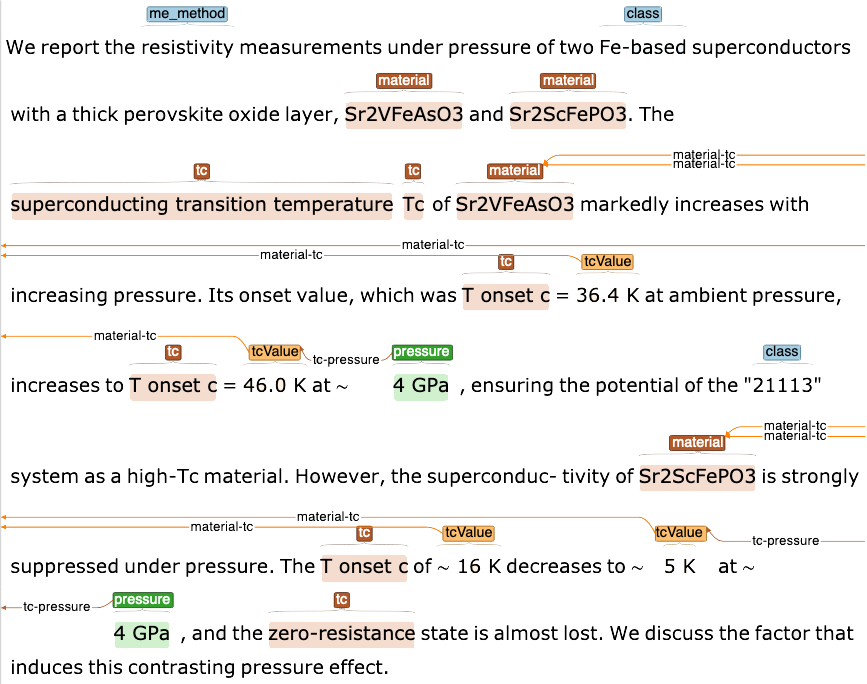
\includegraphics[width=\linewidth]{example-annotated-corpus-postprocess.png}
  \caption{Example of annotated corpus. The example is taken from~\cite{Kotegawa2009ContrastingPE}.}
  \label{fig:example-annotations-and-links}
\end{figure}

\begin{figure}[htb]
    \centering
    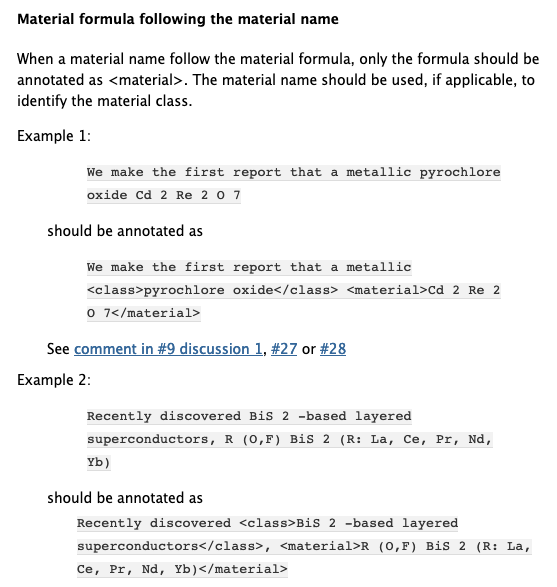
\includegraphics[width=0.9\linewidth]{example-guidelines-1b.png}
    \caption{Example of a snippet of the guidelines. Each tag's description is further divided in several sub-sections discussing specific cases. They are supported with examples and discussions. We use a set of simple XML (eXtended Markup Language)\protect\footnote{\protect\url{https://www.w3.org/TR/xml11}} tags to describe the annotations.}
    \label{fig:guidelines-example}
\end{figure}

\begin{table}[ht]
    \centering
    \begin{tabular}{ | c | c| c| } 
    \hline
        \textbf{Iteration} \# & \textbf{IAA} & \textbf{IAA by label}  \\ [0.5ex] 
    \hline
        1  & 0.45
        &\begin{tabular}{  c | c  } 
            \texttt{<material>} & 0.45\\ 
            \texttt{<tc>} & 0.56\\
            \texttt{<tcValue>} & 0.50\\
            \texttt{<doping>} & 0.21\\
        \end{tabular}    
        \\ 
    \hline
        2 & 0.65
        &\begin{tabular}{  c |  c  } 
            \texttt{<material>} & 0.75\\ 
            \texttt{<tc>} & 0.85\\
            \texttt{<tcValue>} & 0.85\\
            \texttt{<doping>} & 0.39 \\
        \end{tabular}          
        \\ 
    \hline
        3 & 0.89
        & \begin{tabular}{  c | c  } 
            \texttt{<material>} & 0.89\\ 
            \texttt{<tc>} & 0.91\\
            \texttt{<tcValue>} & 0.88\\
            \texttt{<doping>} & 0.94\\
        \end{tabular}       
        \\ 
    \hline
    \end{tabular}
    \caption{Summary of the IAA for each annotation iterations.}
    \label{table:summary-iaa}
\end{table}

\begin{figure}[htb]
    \centering
    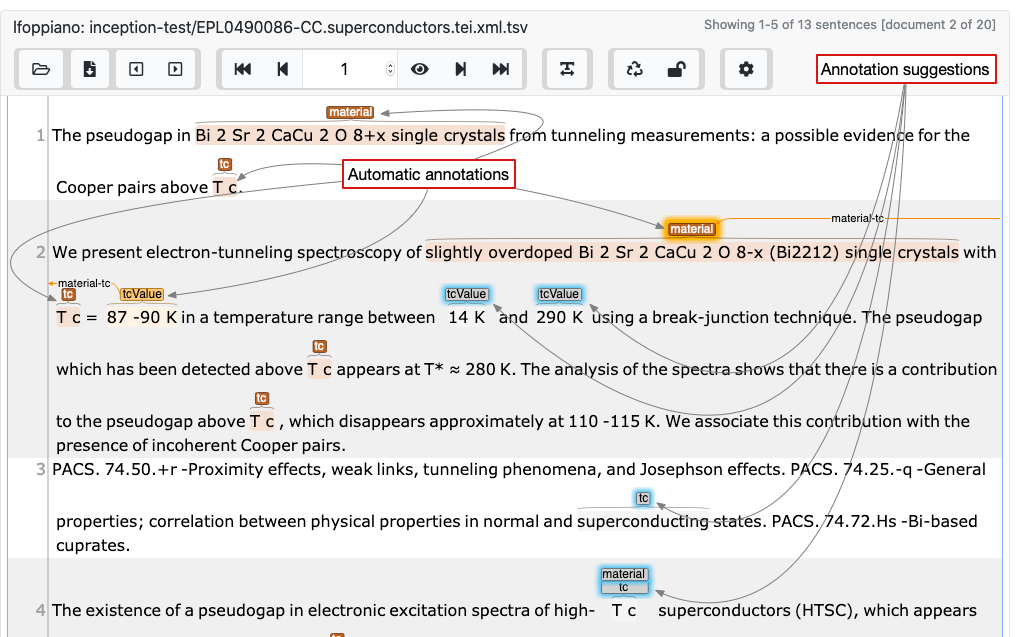
\includegraphics[width=\linewidth]{example-suggestions.png}
    \captionof{figure}{Example of how automatic annotation and suggestions are appearing to the user. The automatic annotations are and look like normal annotations, while the suggestions are not applied by default unless the user click on them explicitly. The example is taken from~\cite{Mourachkine2000ThePI}.}
    \label{fig:example-automatic-suggestions}
\end{figure}

\begin{figure}[htb]
    \centering
    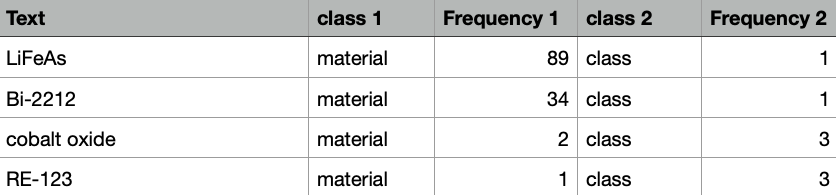
\includegraphics[width=\linewidth]{example-inconsistencies-doubious-mistakes.png}
    \captionof{figure}{Inconsistencies resulted from material and class overlapping. }
    \label{fig:dataset-inconsistencies-unclear}
\end{figure}
 
\begin{figure}[htb]
    \centering
    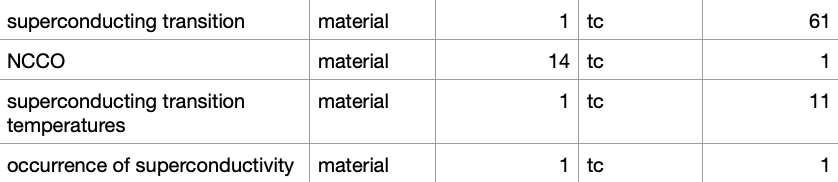
\includegraphics[width=\linewidth]{example-inconsistencies-clear-mistakes.png}
    \captionof{figure}{Inconsistencies resulted from human mistakes.}
    \label{fig:dataset-inconsistencies-clear}
\end{figure}

\begin{figure}[htb]
\centering
  \centering
  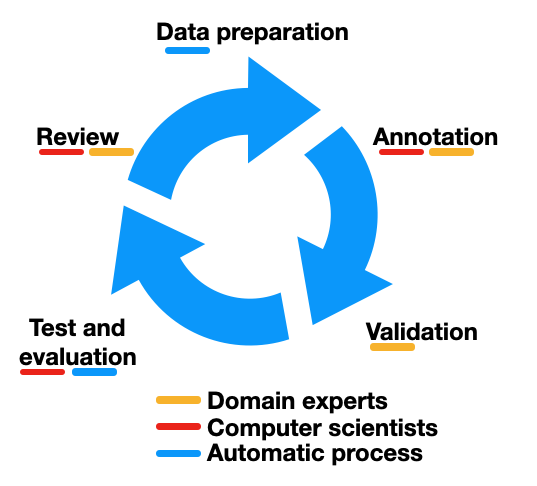
\includegraphics[width=0.5\linewidth]{workflow-schema}
  \caption{The annotation workflow. Different colours illustrate the involvement of each group at each step of the workflow.}
  \label{fig:schema-comparison-modified-workflow}
\end{figure}

\begin{figure}[htb]
    \centering
    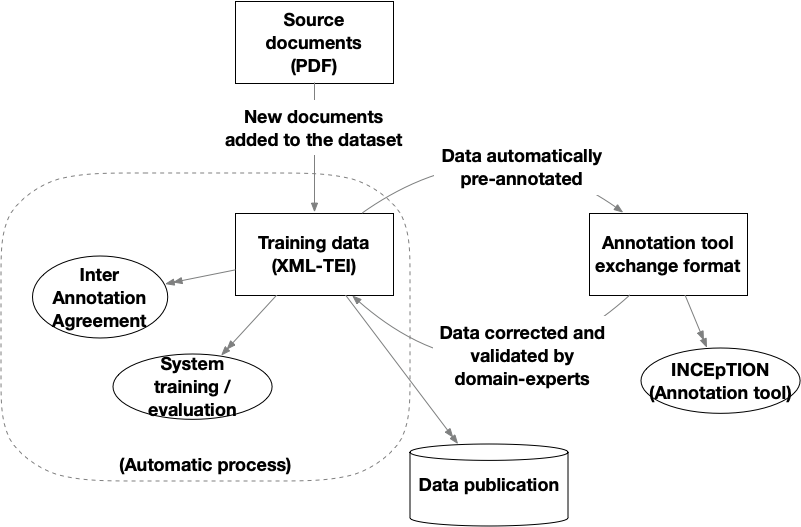
\includegraphics[width=\linewidth]{data-transformation.png}
    \captionof{figure}{Summary of the data transformation within the proposed system.}
    \label{fig:data-transformation}
\end{figure}

\begin{figure}[ht]
    \centering
    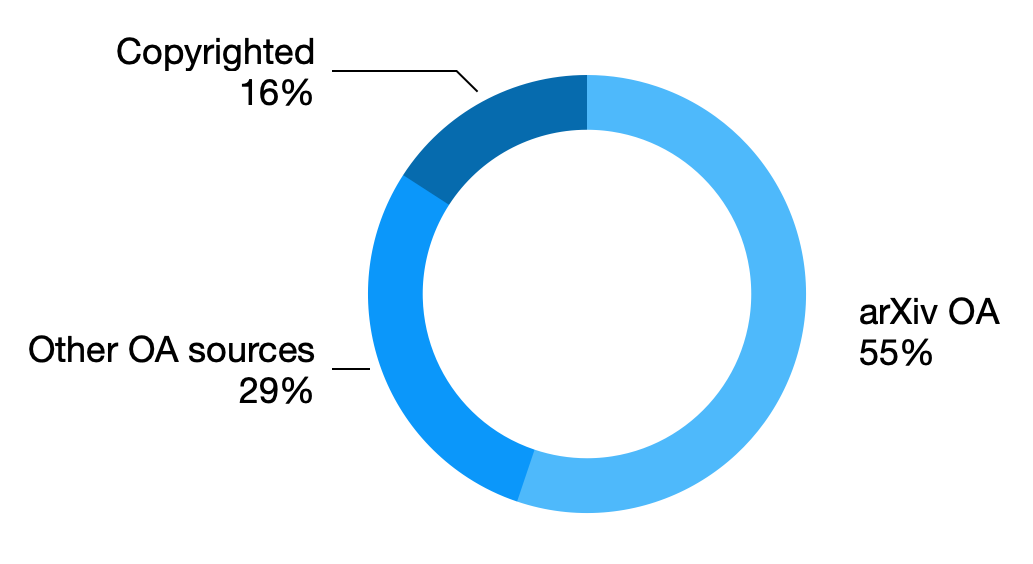
\includegraphics[width=0.7\linewidth]{papers-by-sources.png}
    \captionof{figure}{Papers distribution by Licence (Open Access vs Copyrighted).}
    \label{fig:arxiv-rate}
\end{figure}

\begin{figure}[ht]
% \centering
\begin{subfigure}{0.5\textwidth}
     \centering
    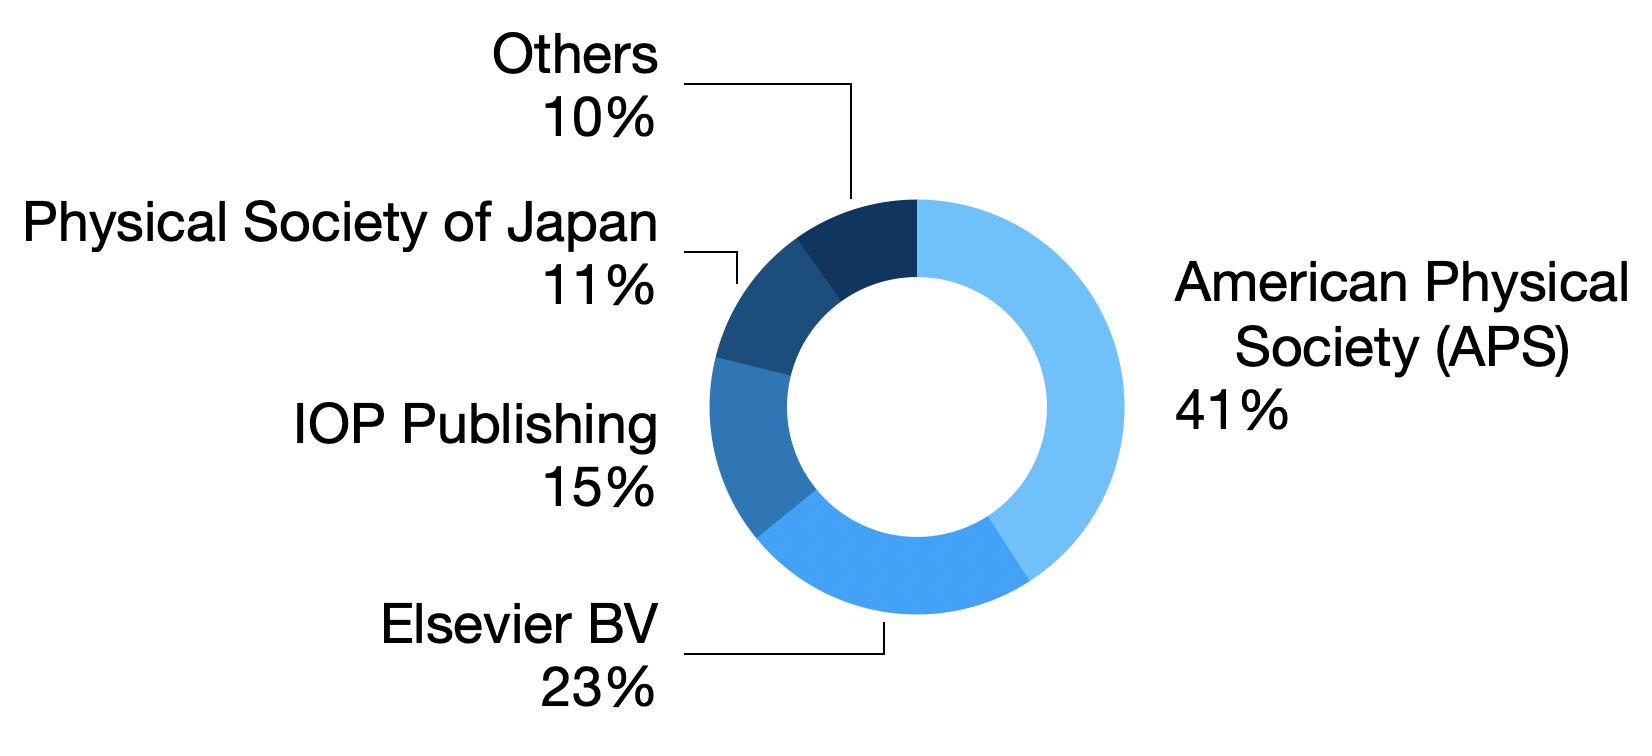
\includegraphics[width=\linewidth]{papers-by-publishers.png}
    \captionof{figure}{Distribution by publishers.}
    \label{fig:distribution-by-publisher}
\end{subfigure}
\begin{subfigure}{0.4\textwidth}
\centering
    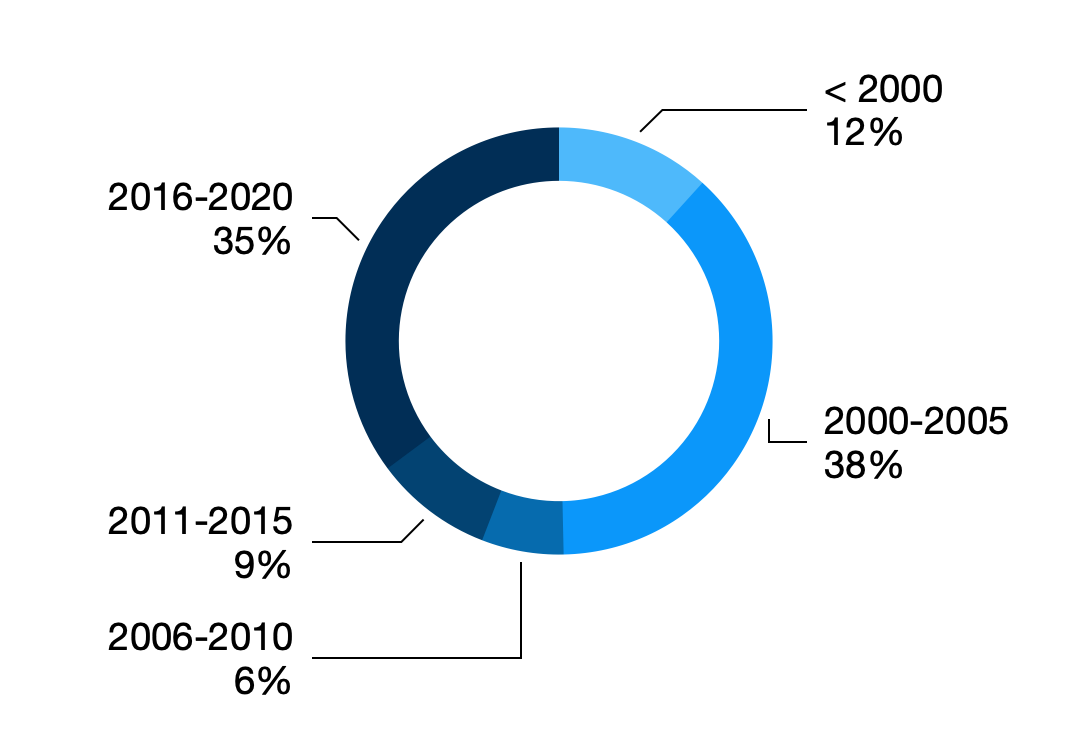
\includegraphics[width=\linewidth]{papers-by-years-donut.png}
    \captionof{figure}{Distribution by years of publication.}
    \label{fig:distribution-by-year}
\end{subfigure}
\caption{Dataset distribution by years and publishers, automatically extracted from the PDF, and consolidated through a lookup to Crossref. }
\label{fig:dataset-distributions}
\end{figure}

\begin{figure}[htb]
    \centering
    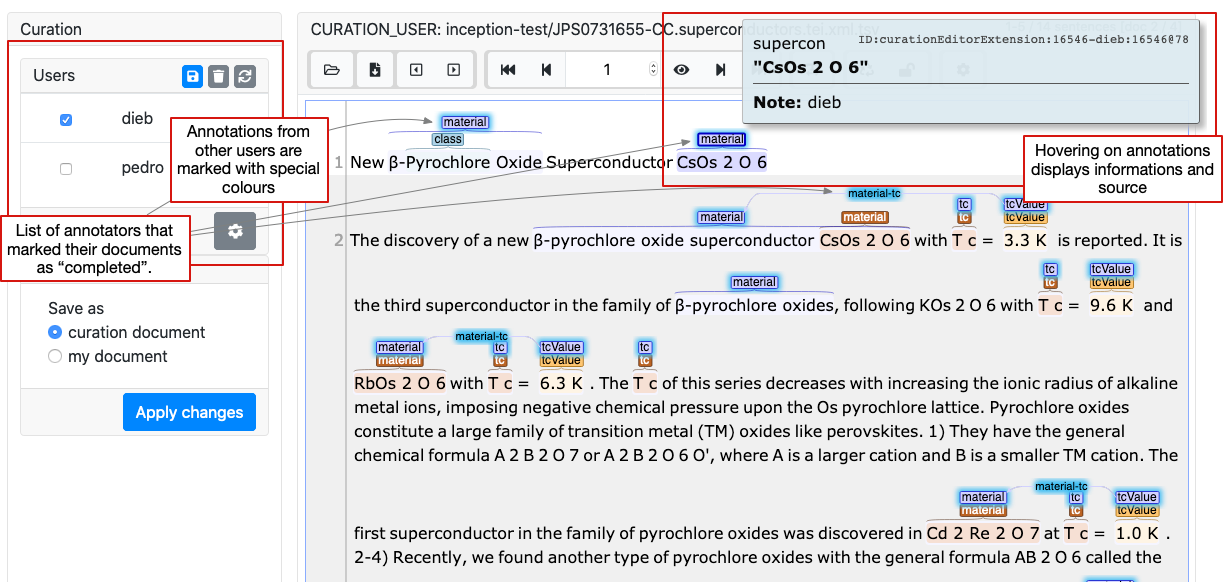
\includegraphics[width=\linewidth]{inception-curation-new.png}
    \captionof{figure}{INCEpTION curation interface. The example is taken from~\cite{Yonezawa2004NewO}.}
    \label{fig:inception-curation-interface}
\end{figure}

\begin{table}[ht]
    \centering
    \begin{tabular}{ |m{6em}  | m{4em} | m{6em} | m{7em} | m{6em} |} 
    \hline
        \multirow{2}{5em}{\textbf{Documents}} & \textbf{Files} & \textbf{Paragraphs} &	\textbf{Sentences} & \textbf{Tokens}\\
         & 114  &	2332 & 	14955 & 	4664\\
    \hline\hline
        \multirow{2}{5em}{\textbf{Entities}} & \textbf{Entities} &  \multicolumn{2}{|c|}{\textbf{Unique entities}} &  \textbf{ Labels} \\
        & 9966 &  \multicolumn{2}{|c|}{4000} &  6 \\
    \hline\hline
        \multirow{2}{5em}{\textbf{Links}} & \textbf{Links} & \multicolumn{2}{|c|}{\textbf{Links\textsubscript{ip}}} 
        & \textbf{Links\textsubscript{ep}}\\
        & 567  & \multicolumn{2}{|c|}{532}&	34	\\
    \hline
    \end{tabular}
    \caption{Statistical overview of the dataset. They are divided into three main groups: Document, Entities, and Links statistics.
    Links\textsubscript{ip} (intra-paragraph) indicate the number of links within the same paragraph. Links\textsubscript{ep} (extra-paragraphs) indicate the number of links from different paragraphs.  }
    \label{table:summary-content}
\end{table}

\begin{table}[hbt]
    \centering
    \begin{tabular}{ | c | c | c | c | c | c | c | c | } 
    \cline{2-7}
    \multicolumn{1}{c}{} & \multicolumn{3}{| c |}{\textbf{CRF}} & \multicolumn{3}{ c |}{\textbf{BidLSTM+CRF}} \\
    \hline
        \textbf{Label} & \textbf{Precision} & \textbf{Recall} & \textbf{F1} & \textbf{Precision} & \textbf{Recall} & \textbf{F1} \\
    \hline
        \texttt{<class>}        & 74.48 &   67.46 & 70.7  & 63.13 & 61.69 & 62.34  \\
        \texttt{<material>}     & 77.95 &   75.38 & 76.63 & 74.48 & 76.69 & 75.56  \\
        \texttt{<me\_method>}   & 63.78 &   59.5  & 61.47 & 66.53 & 74.69 & 70.34  \\
        \texttt{<pressure>}     & 63.13 &   41.46 & 49.05 & 65.96 & 75.00 & 69.89  \\
        \texttt{<tc>}           & 79.17 &   73.71 & 76.33 & 78.17 & 76.72 & 77.41  \\
        \texttt{<tcValue>}      & 74.82 &   66.26 & 70.11 & 69.53 & 76.64 & 72.77  \\
    \hline
        \textbf{Micro avg}      & 75.86 & 71.2  & 73.45 & 72.61 & 74.84 & 73.71 \\
        \textbf{Macro avg}      & 72.22 & 63.96  & 67.38 & 69.73 & 73.57 & 71.39 \\
    \hline
    \end{tabular}
    \caption{Quantitative evaluation of a sequence labelling machine learning model.}
    \label{table:evaluation-machine-learning}
\end{table}

\begin{table}[h]
    \centering
    \begin{tabular}{ | c | c | } 
    \hline
        \textbf{Label} & \textbf{Average}\\
    \hline
        \texttt{<material>}     &   0.946   \\
        \texttt{<me\_method>}   &	0.881   \\
        \texttt{<pressure>}     &	0.768   \\
        \texttt{<class>}        &	0.892   \\
        \texttt{<tcValue>}      &	0.856   \\
        \texttt{<tc>}           &	0.819   \\
    \hline
        \textbf{Micro average}        &	0.896	\\
    \hline
    \end{tabular}
    \caption{Average IAA between annotated and validated documents, over all the dataset [TODO: update table including batch 1, which is still due to be validated]}
    \label{table:average-iaa}
\end{table}

\begin{table}[h]
    \centering
    \begin{tabular}{ | c | c | c | c | c | } 
    \hline
        \textbf{Label} & \textbf{Non-domain experts} & \textbf{Domain experts} & \textbf{Novices}\\
    \hline
        \texttt{<material>}     &   0.924   &   0.969   &   0.924   \\
        \texttt{<me\_method>}   &	0.807   &	0.890   &   0.901   \\
        \texttt{<pressure>}     &	0.72    &	0.836   &   0.746   \\
        \texttt{<class>}        &	0.802	&   0.990   &   0.899   \\
        \texttt{<tcValue>}      &	0.734	&   0.895   &   0.841   \\
        \texttt{<tc>}           &	0.771	&   0.874   &   0.830   \\
    \hline
        \textbf{Micro average}        &	0.857	&   0.940   &   0.896   \\
    \hline
        \textbf{\# paragraphs}  &	423	    &   343     &   325     \\
    \hline
    \end{tabular}
    \caption{IAA calculated between annotations produced by non-domain experts, domain-experts and novices, and the final validated version. The data from non-domain experts and domain-experts has been sampled to provide comparable results. Annotation performed by one domain expert is validated by a different one. }
    \label{table:comparison-iaa-nde-de}
\end{table}

\end{document}
